\section{Background}
\subsection{Problem Context}
This problem's main focus is the difficulty of organising classical sheet music, and how this can be made easier by the automatic extraction of key pieces  of information. In order to understand what a performer may want to know about a particular piece, it is important to have a brief understanding of the elements of musical notation common to all compositions.

The key element of this form of notation is the staff, as shown in figure \ref{fig:staff}. This is a grouping of five horizontal lines, with each line or space in the staff indicating a different sound pitch, a term meaning the relative "highness" or "lowness" of the sound \parencite{classroom}.

\begin{figure}[h]
    \centering
        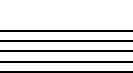
\includegraphics{staff-crop.pdf}
    \caption{A blank staff}
    \label{fig:staff}
\end{figure}

This staff is divided by bar lines, vertical lines delineating grouped units of sound and silence (formally referred to as notes and rests), which provides an indication of the unit's relationship in time by its juxtaposition to other groupings in the composition. These groupings are called measures or bars, with each bar having a variable maximum of notes and rests. 

\begin{figure}[h]
    \centering
        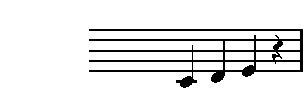
\includegraphics{bar_with_notes-crop.pdf}
    \caption{A bar containing three notes and one rest}
    \label{fig:staff-notes}
\end{figure}
\subsubsection{Clefs}
In the system of staff notation, sound frequencies, or pitches, are denoted by letters A-G - after each cycle of the letter names, the next pitch above it will be the start of a new cycle. The cycles are often split by octaves, a term meaning eight pitches, for example A to A or E to E. 

In order to provide a link between the lines and spaces of a staff and the pitch names, a clef symbol is necessary.
\begin{figure}[h]
    \centering
        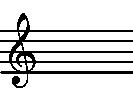
\includegraphics{clef-crop.pdf}
    \caption{A staff with a treble clef}
    \label{fig:clef}
\end{figure}

Each clef symbol denotes a different pitch name - figure \ref{fig:clef} shows a G. The center around which this symbol is drawn - in figure \ref{fig:clef}, the second line from the bottom of the staff - indicates that this line or space will be known as the pitch name denoted by the symbol. From this the reader can infer all other pitches by counting through the letters of the cyclic octave system, so in figure \ref{fig:clef}, the space above becomes an A, and the space below becomes an F.

This symbol is important to a musician as different clefs are used to position the majority of the pitches in a piece on the staff, as this makes it easier to read. From this a performer can infer the average range of a piece, and predict whether this will be comfortable for the performer's chosen instrument or voice.

\subsubsection{Keys}
A second important indication to the player is the key, denoted by a key signature.
\begin{figure}[h]
    \centering
        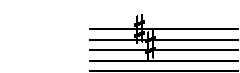
\includegraphics{key-crop.pdf}
    \caption{A staff with a key signature}
    \label{fig:key}
\end{figure}

The key signature is a collection of symbols at the beginning of the piece which indicate which pitches should be raised by half pitches, and which should be lowered. Raised pitches are called sharps, indicated by the \# symbol, whilst lowered pitches are called flats, indicated by the $\flat$ symbol. Each key, which has a letter name and key type (which can either be "major" or "minor"), has a different combination of flats or sharps. All pieces have a key, regardless of whether there are any flats or symbols notated here. In the case where there is no key signature, the piece is in one of two most common keys - C major, or A minor.

This is a useful piece of notation to a musician as pieces in less common keys, such as C\# major or F\# major, may prove more difficult for the user to perform, and therefore they may want to filter out pieces in these particular keys. Similarly, in the case of singers, a singer's range may sit comfortably in one or two keys and they would perhaps want to find pieces in only these keys. 

\subsubsection{Meter}
The third symbol denoted at the beginning of a measure is the meter or time signature, displayed as two numerals positioned like a mathematical fraction.

\begin{figure}[h]
    \centering
        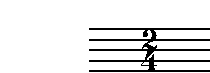
\includegraphics{meter-crop.pdf}
    \caption{A staff with a 2/4 time signature, or meter}
    \label{fig:meter}
\end{figure}

The upper number of a meter symbol indicates the amount of beats in the bar. A beat simply refers to a note or rest, and the type of beat is indicated by the lower number. In the case of figure \ref{fig:meter}, 2/4 indicates a measure will contain 2 quarter notes. The most common time signature is 4/4, which for this reason is usually denoted with a C in place of the fraction, meaning "Common time".

This information is important as it tells the performer how the rhythm and beat of the piece should be felt, counted and performed, and is useful for searching purposes as different meters give the piece a different feeling, dictating the sort of occasion this piece would accompany. 

For example, 2/4 is commonly used for march pieces, and 3/4 is commonly used for waltzes and dance pieces.

\subsubsection{Tempo}
The speed of a particular piece, or the tempo, is indicated by an equation.

\begin{figure}[h]
    \centering
        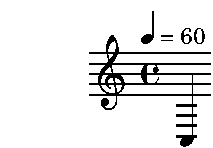
\includegraphics{tempo-crop.pdf}
    \caption{A staff with tempo marking}
    \label{fig:tempo}
\end{figure}

The equation above the staff in figure \ref{fig:tempo} indicates that the piece should be played at 60 beats per minute. The symbol dictating the sort of beat per minute depends on the time signature, here a crotchet (or quarter note) is given as the piece is in 4/4 time. Sometimes, this will be accompanied by a text direction to indicate speed or style, such as Andante, indicating a walking speed.

This indication would prove a useful identifier as pieces of different tempos provide variation in performance lists, so a concert organiser may want to find pieces with a variety of tempos.

\subsubsection{Further metadata}
Aside from these symbols, there are some items of textual information useful to the user. 

The first of these would be the parts in the piece and their transpositions. A part refers to a grouping of measures given to one performer, as shown in figure \ref{fig:parts}. "Part" used in a general sense usually refers to the names given to the left, in this example, "Clarinet in B$\flat$" and "Flute".
\begin{figure}[H]
\centering
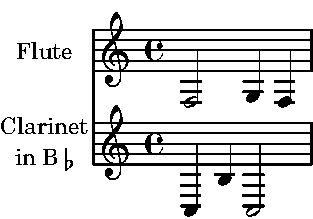
\includegraphics{multiparts-crop}
\caption{Two separate parts in one score}
\label{fig:parts}	
\end{figure}

Parts would be relevant as a particular group of instrumentalists may need parts that fit their instruments. If this is not the case for a given piece, however, a part written for a different instrument, for example, the Alto Saxophone rather than the Tenor Horn, may be compatible with the instrument anyway, if the transposition matches the instruments together. 

An instrument which has a transposition means that, whilst most instruments would play a note as it is written, a transposing instrument will automatically sound the note in a different key, as described earlier, which may raise or lower the sound of the note. For example, the note C played on an Alto Saxophone will sound as an E$\flat$, because it is in the key of E$\flat$ major. 

Further to this, the user would want to know the piece's title, and names of publishers, composers, arrangers and lyricists of the work, commonly known as the bibliography of a piece \parencite{MIR}. Further to the composer name, it may be useful to know the date of composition as an indication of the era in which the piece was composed, such as Classical/Baroque/Romantic, though this would not always be written on the sheet music so may need to be researched using the Internet.

\subsubsection{Sight Reading and Difficulty Grading}
This portion of the problem context relates to the difficulty grading secondary objective. It is important to understand why this would be useful to a musician, and as such what follows explains some more specific technical terms which a musician may use to assess pieces of music.


Difficulty grading is a subconscious act which takes place during the initial phase of learning a piece of music. This phase is often referred to as "sight reading", a term meaning that the performer has had little to no practice in performing the sheet music. %todo ref
 It is referred to as sight reading because the musician can only perform symbols as they occur in the music, or as the reader sees the symbols. They may not be familiar with where and when these symbols occur, how and at what speed to perform certain note patterns are to be played, or what keys are to be applied at specific points in the music. The lack of practice can contribute to the performer playing the piece hesitantly, or with mistakes.

After more practice, a performer will generally gain muscle memory of certain repeated note sequences and be more aware of what changes are coming up without needing to read the music. In some instances a performer may memorise a piece of music through repeated practice without consciously intending it. 

In order to gauge whether it will be worth sight reading a piece of music, the performer will often visually and subconsciously assess the music for difficulty. This is generally subjective, depending on the level of confidence and ability of the performer, and can change depending on the chosen instrument. However, there are some elements of music which affect this grading for all musicians.

Examples are a note or rest of a very short duration in a fast tempo, particularly in sequence with other short notes. An example is given in figure \ref{fig:notesequence}, wherein the notes are a 16th of the duration of a quarter note, and the tempo is 180 quarter notes per minute, indicating 3 quarter notes should be played per second.

\begin{figure}[H]
\centering
\includegraphics{quick-notesequence-crop}
\caption{A rapid sequence of demi semi quavers, (a quarter of an eighth note in duration)}
\label{fig:notesequence}	
\end{figure}

 This is considered difficult because it is hard to ensure that the duration of each note is precise, and in sequence it can be difficult to ensure that the performer can fit all of the notes into the pattern with precision. Often these sequences can cause a performer to blur the notes together, meaning that one note is indistinguishable from another, and may not even be heard if the performer has not timed the note correctly.

Further examples relating to pitch in a general sense are notes which are at the high or low end of an instrument's range, which for reeded wind instruments can be uncomfortable due to changes to embouchure. Reeded refers to a family of instrument whose sound is produced by vibrating a piece of very thin wood against something whilst blowing air through the vibration. Embouchure means the grip or tightness of the jaw. In combination with the airflow, this pressurised grip against the reed is what causes it to vibrate.

Performers who play reeded instruments control tone and pitch by tightening or loosening their embouchure. In the case of notes at the top of an instrument's range, this can be uncomfortable as it requires tightening the teeth against the lips, a position the performer's mouth may not be accustomed to, and in the case of notes at the bottom of an instrument's pitch range, it can be difficult to achieve due to loosening their jaw being more of a subconscious act which requires practice to achieve the right level of jaw release. In addition to the difficulty of "pitching" the note correctly, it can be hard to jump between notes due to the rapid change needed in embouchure pressure.

For string instruments, particularly those without frets indicating the position of specific pitches, it can be difficult to play the notes on the edges of their instrument's range with precision due to lack of practice, as these notes are not always in common usage. Lack of practice on any instrument can cause the sound to be uncomfortable to listen to due to subtle differences in pitch which the human ear can pick up, meaning that a musician will dislike practicing a lesser used note if it is not completely necessary.

Complex rhythms, a term referring to the different durations of a particular sequence of music, can also cause difficulties, particularly for instruments like the piano in which the player has to play in polyphony. Polyphony means multiple sounds or lines of note sequences. In the case of a piano player, it is common for pieces to present cross rhythms in which the left hand and right hand are not playing the same rhythm, and precise timing is required to get the rhythms synchronised with each other. 

An example of this is figure \ref{fig:crossrhythms}. Here the right hand plays two quarter notes, whilst the left hand plays three eighth notes. The three above the eighth notes indicates that the pianist must fit the three notes into the same time sequence as one quarter note, known as a "triplet" because the player must fit three notes into a time space where there would normally only be two.

\begin{figure}[H]
\centering
\includegraphics{crossrhythm-crop}
\caption{A cross rhythm}
\label{fig:crossrhythms}	
\end{figure}

The developer has assessed this area with some detail, and results from a survey of other musicians with varying level of ability as well as chosen instruments, with some analysis of other factors are given in the appendix.

\subsection{Comparison of Technologies}
\subsubsection{Programming Language}
This project could be developed with a variety of programming languages, as displayed in table \ref{table:langs}.

\begin{table}[H]
\centering
\begin{tabular}{| l | l | l | l |} \hline
  {Language} & {Speed of development} & {Developer's Knowledge} & {Most recent use} \\ \hline
  C\# & Fast & A lot & 2nd year \\ \hline
  C++ & Slow & Average & 2nd year \\ \hline
  Python & Fast & A lot & In constant use for over a year \\ \hline
  
\end{tabular}
\caption{Table of languages considered}
\label{table:langs}
\end{table}
The first language in consideration is C\#. C\# is mostly used on Windows due to the main compiler being closed source and developed by Microsoft, but with some platform independence due to the Mono Project, which is feature-complete to C\# 10 \parencite{MonoDev}. There are several other possible tools to create applications for other operating systems using C\#, such as Xamarin Studio, but the developer has not developed any applications with C\# for use on multiple operating systems. 

In terms of speed of development, the developer considers that the language syntax is reasonably intuitive and consistent. However, as C\# is statically typed, this means that rapid prototyping is slower due to more keystrokes and needing to be completely aware of return types for methods at all times.

Finally, due to the language being mostly for Windows and largely being closed, C\# has a lower amount of Open Source projects on the popular Open Source Code Repository Github \parencite{Redmonk}, as shown by the graph in figure \ref{fig:graph}. Whilst this is not necessarily important to development at this stage, the developer intends to Open Source the project and if there is a lower percentage of repositories for this language, that could potentially indicate a lower number of contributors.

\begin{figure}[h]
\centering
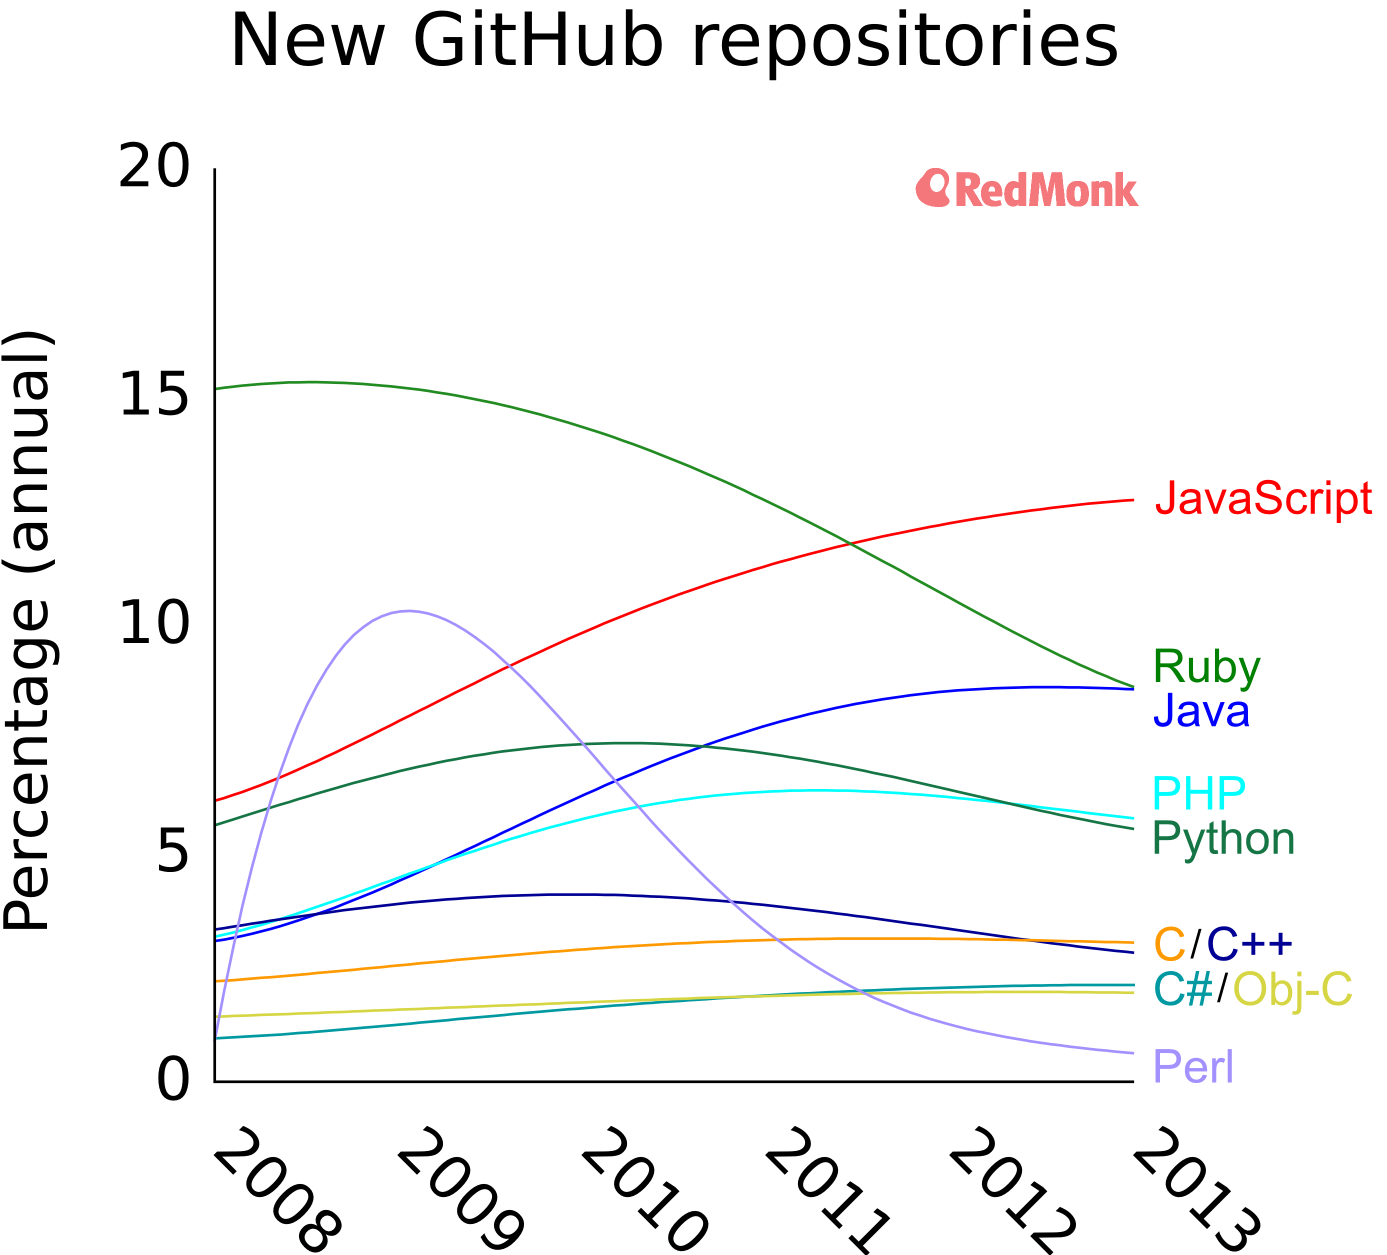
\includegraphics[width=250pt]{github-repos}
\caption{A graph showing the percentage of repositories on Github in different languages \parencite{Redmonk}}	
\label{fig:graph}
\end{figure}
The second language in consideration is C++. Whilst C++ is arguably the closest to native code and therefore the language which will be the best for cross platform development, the syntax and memory management issues of C++ mean that development can be slower, particularly when the developer does not feel as competent using this language.

The third language in consideration is Python. Python is cross platform, as it is included by default in OSX and Linux based Operating Systems with the ability to install it on a Windows operating system.

In terms of development speed and syntax, Python's syntax is the closest of the three considerations to english or pseudocode, and thus requires the least amount of key strokes. Being closer to english also means that the project is more likely to attract a wealth of less technical contributors, in particular musicians, as the language should be easier to learn how to use.

 Furthermore, as it is dynamically typed this allows the developer to use a particular advantage of duck typing whilst developing, meaning that so long as a class has a particular behaviour, the program can use the class for it's purposes and ignore differences to other classes without implementing an interface.
 
 As exemplified by the graph in figure \ref{fig:graph}, Python has a higher percentage of new Github repositories. Again, this does not indicate that Python is the best language for Open Source as that hypothesis would be hard to objectively prove, but it does potentially indicate a higher number of available developers with knowledge of Python when the project is open sourced.
 
 Lastly, there are many current projects written in Python in the area of music research \parencite{pmus}, which means the project will be easier to integrate and communicate with other projects or build upon the work of others without needing to port software to Python.

It is for these reasons that Python has been chosen as the development language. Beyond the selection of Python, it is important to discuss and consider which version to use, as Python 3 was introduced in 2008, but Python 2.7 continues to be maintained and was updated to include many of the backwards compatible features in 2010. Whilst this seems an obvious choice as Python 3 is the latest version, many projects still have issues updating and using Python 3 as it was deliberately not backwards compatible \parencite{Foundation2}.

Upon due consideration, Python 3 has been selected. This decision has been made because the project does not require any libraries which are not available for Python 3, and therefore the developer should make every effort to keep the project up to date with the latest version.

\subsubsection{File format}
The project will require at least one default format for it to process music, which needs to have detailed information about what the score contains. This is necessary for information extraction and for the generation of readable sheet music. Table \ref{table:formats} describes the options considered.

\begin{table}[H]
\centering
\begin{tabular}{| c | c | } \hline
  {\textbf{Format}} & {\textbf{Purpose}} \\ \hline
  new format & this project only \\ \hline
  muscx & MuseScore notation \\ \hline
  SIB & Sibelius notation \\ \hline
  MusicXML & sharing music between software \\ \hline
\end{tabular}
\caption{A table showing the different file formats considered}
\label{table:formats}
\end{table}
The first option is to create an entirely new format. This would mean the file format was designed to the requirements of the project and therefore would be entirely customisable and extensible. However, this would require further design into how the file would be structured, loaded and unloaded.
 It would also not be implemented as standard to software which composes music, and as such would either require manual file creation or require writing a conversion script for files of other formats. This project is created with the intention of organising, not composing music, therefore creating an entirely new format would be considered a drain on the developer's time when other formats which are more standardised could be implemented without conversion scripts.

The next two options, muscx and SIB files, are formats used by the open source composition software MuseScore \parencite{MuseTour}, and the world's most popular proprietary composition software, Sibelius \parencite{avid}. Using either or both of these files would mean the majority of users would be able to use the application. 
However, both formats would couple this project with those particular packages, when users could still choose other software to write music with. Furthermore, the formats are specifically designed for those software packages and may have nuances which make development for this project more difficult. Additionally, Sibelius is proprietary so borrowing their file format may cause copyright issues.


The fourth and final option is MusicXML, a file format intended for sharing and archiving the world's sheet music \parencite{mxml}. This particular format is used by a wide variety of software packages \parencite{mxml} and is included in the formats usable by both MuseScore \parencite{MuseTour} and Sibelius \parencite{avid}. Using MusicXML would avoid coupling the format with a program and would not require manual creation or import of current music files. 

Aligning the project with an open format like this will make the project a better renderer, as the project will be designed to handle MusicXML more effectively than other packages which are designed to use their own format by default, then import or export to MusicXML. This method of storing and loading data is used by MuseScore, and comes with several issues and problems as well as inconsistencies, as documented in their issue tracker \parencite{mscoreBugTracker}.

However, this particular format was designed by a third party, Make Music, who have a vested interest in the file format and it's structure as they produce Finale, another popular music editing package \parencite{mxmlSoft}. This means that the design aims of the file format have a particular alignment to that platform, and will not necessarily be logical to work with.

Using MusicXML also means that there will be a technical challenge of learning how to use and understand the format, which may affect the development time adversely if the developer does not pick up enough initial knowledge to design the system effectively.

For reason of inclusion in composition software packages, MusicXML has been selected as the file format for the project. 

\subsection{Comparison of Technologies for Rendering Music}
Figure \ref{fig:flow} shows the flow of data into and out of the system in order to produce a working renderer. Each stage of this process will be discussed in detail in the following sub sections.

\begin{figure}[H]
	\centering
	\includegraphics[width=80pt]{diagrams/flow-rendering-crop}
	
	\caption{A flow diagram describing the process of rendering sheet music from XML}	
	\label{fig:flow}
\end{figure}

\subsubsection{XML verification Considerations}
Before XML is parsed for information in the flow chart in figure \ref{fig:flow}, the file is by default validated using the DTD defined in the XML file, which can optionally be switched off by the developer. Whilst this confirms that XML is valid before starting to parse a file which could be corrupt, the speed at which files will parse is greatly reduced according to the speed of the user's internet connection.

Furthermore, if the user is browsing their own music collection, it should not be necessary for the user to be connected to the internet.

Due to speed and functionality considerations, the choice has been made that the XML parser algorithm will not verify XML before beginning to parse it. Given that most musicXML will be produced automatically by other programs, it is unlikely files opened by the project will be corrupt, though necessary steps will be taken to avoid this causing a problem in the program.


\subsubsection{Libraries for parsing XML for information}
In order to extract information from each tag in an XML file, there are two potential built in methods to choose from. 

The first, known as DOM or Document Object Model, loads the entire XML file into memory and provides methods to search the loaded file for specified tags \parencite{PythonDom}. The developer has used the Python DOM library before in personal and industrial projects, and believes it is cumbersome to manipulate data in this way. Furthermore, this project is focussing on rendering the information rather than rendering it with precise formatting, and many software packages implant musicXML files with very complex formatting information which may or may not be necessary \parencite{MusicXMLPresentation}.

The second option is using a different api called the Simple API for XML (SAX). In this method, the library will load the XML file tag by tag, and connect to developer-defined call backs when specified things occur in the file, for example a new tag or piece of data inside tags, or the closing of an old tag \parencite{PythonSax}. 

This is easier to work with as functionality can iteratively be built up by creating handlers for each tag, and is better for memory management as only tags which are necessary to the project will have any effect on the program or program memory. For these reasons, this method has been selected.



\subsubsection{Algorithms for display and storage of XML information}
For the rendering of sheet music, the system must in some way manipulate the data extracted from the XML file into a visual output.

The usual method of formatting an XML file would be applying an XSL stylesheet, which is commonly the method of choice for rendering XML files in a web browser. This is not an option in MusicXML because the notation is too complicated and requires too many symbols, whilst XSL stylesheets are usually used for images and text representations. Sheet music is somewhere in between the two, and thus this option cannot be selected.

The second option would be to create or reuse a converter script from XML to the output format, meaning the output would be generated at the same time as the input. However, this couples the system with MusicXML and would slow down development if it were required to use a different additional input, or decisions were made to change the output format. Furthermore, the Big O representation of this type of script to any output format is $O(n^2)$, which is not a highly optimised algorithm.

The final option is to create a converter script which would parse the MusicXML and create a hierarchy of objects. This avoids coupling directly to MusicXML as new formats of both input and output would only need a converter script to create object hierarchy or from the hierarchy to the output format. The big O representation of this particular method is $O(n)$, a noticeable improvement on the converter script option.

However, whilst this avoids coupling, a technical challenge is created using this method in that the object structure needs careful planning to cater for the structure of MusicXML and the structure or method of output, which, with little knowledge of the input or output format, is difficult to achieve.

Parsing to objects has been selected as the method of choice in order to avoid coupling and create an extensible system.

\subsubsection{Rendering System}
Given the decision made in section 3.3.3, the system must take the object hierarchy and transform it to readable sheet music. The user should be able to pan around the sheet music and zoom in and out of it to view specific details.

This could be achieved using an entirely new system, with the output going directly to the render window using different glyphs and fonts extracted from their relevant classes.

However, the functionality of panning and zooming using this system may be difficult to optimise, as both could possibly require running the system each time the user provides input. 

Furthermore, the conversion of even basic sheet music to a readable format would require a high level of precision and complexity. The time put into creating a new rendering system would be considered unnecessary as this is a process that has been covered by many different applications (like MuseScore \parencite{MuseTour}, Finale \parencite{mxml}, Sibelius \parencite{avid} and Lilypond \parencite{Lilypond}). 
Lastly, the process of debugging whether the symbols are correct would require visual checking and would be difficult to debug automatically.

It would be possible to alleviate the panning and zooming problem by converting the collection of symbols to an image or PDF file and using a built in image rendering library to display this output, such as wxPython \parencite{WX}. However, this method still involves the process of creating an algorithm which has already been covered and adopted by many parties, and incurs problems with visual debugging.

The final option is to output the structure to a formatted file, and have an external rendering system parse this formatted file. Lilypond is a language and system developed to typeset the highest quality sheet music \parencite{Lilypond}, which takes an input file and outputs a PDF or image. An example of some lilypond code is given in figure \ref{fig:lilypond}, with the processing output from Lilypond given in \ref{fig:lilypondrun}, and the resulting pdf given in figure \ref{fig:lilypondres}. As this is a language unto itself and has been in development for many years by the Open Source community, this will alleviate the problem of visual debugging - instead, each class can create a formatted Lilypond output based on its attributes and unit tests can automatically confirm that the result is as expected.

\begin{figure}[H]
\centering
\begin{minipage}{120pt}
\centering
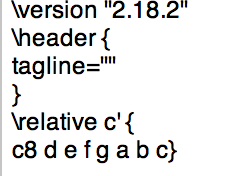
\includegraphics{lilypond}
\caption{An example of Lilypond input}
\label{fig:lilypond}
\end{minipage}	
\centering
\begin{minipage}{300pt}
\centering
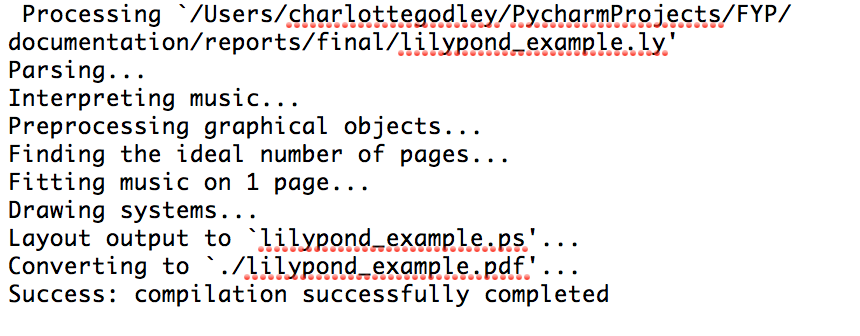
\includegraphics[width=290pt]{lilypond_run}
\caption{The processing output from Lilypond}
\label{fig:lilypondrun}
\end{minipage}
\centering
\begin{minipage}{160pt}
\centering
\includegraphics[width=150pt]{lilypond_example-crop}
\caption{The PDF output from Lilypond}
\label{fig:lilypondres}
\end{minipage}
\end{figure}

There are other options and packages which are part of the \LaTeX\  
 eco system, another typesetting language. This project typesets documents, rather than sheet music alone. The two major packages are MusiXTex and ABC \parencite{musixtex}, but as both of these packages are embedded into \LaTeX\
 which is unnecessary for this particular project, this may bloat the user's operating system with unnecessary software.

The chosen option for the rendering system is to output formatted files to Lilypond, which will then take the output and generate a PDF.

\subsection{Comparison of Technologies for Organising Sheet Music}
This section discusses the organisation of sheet music. This involves parsing and verifying an XML file as explained in 3.4.1, extracting data according to a metadata model as explained in section 3.4.2, and storing it in order to be searched and manipulated, as explained in section 3.4.3. After this process is completed, the user will want to query the data set which will require some processing of an inputted string, explained in section 3.4.4. The decisions taken over all these areas of organising sheet music will be expanded upon in the sections below.
\subsubsection{XML data acquisition algorithm}
This objective, like the rendering objective, takes data from XML files in a folder provided by the user. As such, both objectives require decisions on which method of parsing would be most appropriate - DOM or SAX, and verifying or non verifying.

The system will use SAX because there are only a select few tags and collections of information that the database will need to peruse, and SAX means that only these tags will have an effect on the algorithm or memory.
The file will not be verified before being parsed in order to avoid the need for internet connection, and to speed up the loading and parsing process.

\subsubsection{Metadata Model}
In order for the system to scan a file for data, a model of what data to collect will need to be designed and implemented. In normal circumstances there may be a model already described as standard for the subject area. In the case of music and music research, there are many facets and disciplines which have an interest in collecting data about music \parencite{MIR}. For example, a musicologist may want to study patterns, a sound engineer may want to study instrument timbres and transpositions, or an Artificial Intelligence researcher may want to study the generation of music in a general sense \parencite{creativeMachines}. 

For these reasons, there does not appear to be a standard model, and therefore this project will create a new, general model for music information retrieval.
There are two options in consideration for the model of data to collect.

The first model would collect general symbolic data, such as the elements described in the problem context - time signature, meter, clef, key, instruments, transpositions, and bibliography information. This provides data that will be useful to every musician reading the music, gives a reasonable amount of complexity and variation and allows for a wide range of searches.
However, this does not provide much information which would be useful to specific instrumentalists. For example, a piece containing a lot of pitch movement or certain sequences of notes may prove to be something one instrumentalist wants to avoid, but for another it may be of no consequence.
Furthermore, for the difficulty scanner objective this model would need to be expanded to include note durations and patterns, and apply some semantics to the model to deduce the grading.

The second model would collect data with specifics according to instrument name, and make the parser apply certain rules to deduce what would be useful for each player to know. This provides more precision to the data and has a higher likelihood of being useful data to the user. 

However, this would be more technically challenging due to the need for semantics and specific structuring of data in a way that the first option would not, as the data has a lot more variance from piece to piece and part to part. 

Additionally, relying on the instrument name to deduce rules to apply may be a problem due to different spellings of names which would mean the scanner would have to prepare for all possible changes. For example, some pieces may use plurals to indicate more than 1 instrument should play 1 part, and some pieces may provide the key as well as the instrument or some may use the default which the scanner would have to deduce, like "Clarinet" or "Clarinet in Bb". Another consideration that the scanner would need to make is language, as some human languages name instruments differently, such as gaita which is bagpipes in Spanish. Selecting human languages in the user interface would not solve this problem, as it is common for composers to produce music which contains the instrument names as they are referred to in their native tongue, and it is not common for there to be an available version in any other language.

The developer has decided to use the first option, but design the system so that the parser could be expanded at a later stage of development to allow for piece difficulty ratings to be implemented.

\subsubsection{Memory considerations}
The metadata algorithm will parse all of the files in a given folder which have the XML extension for the model described in the previous section. It will be necessary in some way to store this information, potentially both physically to avoid unnecessary repeat meta data scans, and in memory to allow the program to manipulate the data.

It would therefore be possible to simply extract the data and store it to an in memory object, which would then be loaded and saved to a serialised Python object file. This would be quick to develop as it only requires using the Python serialisation libraries in collaboration with the XML acquisition libraries, and has a simple system design. 
However, the algorithms and overall design of the memory object would mimic much of the functionality of a database, so would be considered duplication of other people's work with little technical improvement. 
Furthermore, any extensions other developers made to improve or change the dataset would have to be written or connect to Python, as this would be the only way to unserialise and understand the outputted file.

The chosen solution therefore is to extract data, then communicate with a database instead of an in memory object. Queries to the database would result in ordered lists of files and tuple data sets which could then be manipulated by the system. 

This is preferable to the earlier suggestion because database systems have been worked on by multiple contributors including several well known companies who support open database architectures with funding and developer time \parencite{SQLiteConsortium}. The invested time of other developers and companies means more time has been spent on optimising the searching and sorting methods, usually through the implementation of a B-Tree file structure \parencite{SQLiteBTree}. For these reasons using a database would most likely have faster access and search times than an in memory object.

Furthermore, using a database avoids coupling any future improvements to Python, as the most common database structures have well designed APIs for the most popular languages \parencite{MySQLAPI}.


\subsubsection{Query Processing Considerations}
The application should allow the user to input a search query and find results which match the input. A user can then select from a list of result options which will render the selected file. In order to deduce what tables and data sets to query based on user input, it will be necessary to structure the query in a certain way.

The first option for achieving this would be to define a querying syntax and provide the user with instructions or a tutorial on how to use this syntax. This allows for a lot of complexity and means that the program will not need to do as much string manipulation and processing.

However, this also makes the program less intuitive to use and could cause users, particularly those who are less technical, to be confused or apathetic to the program if the syntax is too complicated. Furthermore, some searches, such as finding all pieces by Mozart, do not require a high level of complexity as results could be achieved using the word "Mozart" without much context.

Another option would be to allow the user to input anything and try to predict from the input which table to query. This would easily be achievable for text input and for input which has symbols specific to one notation element or another. An example of this would be a time signature, which is the only input which would be represented as a fraction, like 4/4, or perhaps a tempo indication as it would always have an equals symbol in the input.
However, this removes the ability to build up complex queries and for some elements, like clef or key, it would not be possible to deduce merely from text what the user is expecting. This could potentially result in the system querying all tables for the data, or result in excluding some elements of meta data in order to avoid a processing overhead.

The selected option therefore will be an amalgamation of the two described options, which will allow for both simple strings, such as 4/4 or quarter=half when defining time signatures and tempos, and for more complex input, such as instrument:clarinet with:clef:alto. This will enable users to search without needing to know or use too much search syntax and is aimed to be intuitive and simple. Instructions for the querying syntax are provided in the user guide in the appendix.



\subsection{Comparison of Technologies for Importing Online Musical Sources}
The project should be able to search online, using various sheet music collections, for new music for the user. This involves selecting sources to implement in the project, and implementing an algorithm for downloading and parsing files from those sources. In addition to these technical considerations, the sheet music on these sources may have different licensing arrangements, so handling terms and conditions of sheet music usage will also need to be considered, as detailed in section 3.5.3.
\subsubsection{Sheet Music Sources}
The project should be able to communicate with one or more online music catalogs in order to allow the user to expand their collection. Whilst the system should be designed for extendability, at least one source should be integrated to the system to prove functionality.

The source this project focusses on using is \textbf{MuseScore Online}, which is a community website created for composers to upload, share and discover compositions using the MuseScore platform \parencite{MuseShare}.

This has been selected due to the number of files available, the openness of the platform and the well documented API. It will, however, be necessary to manage copyright issues, as pieces published on this website may be published under the license of the composer's choosing and therefore may cause issues with certain types of users, in particular those performing commercially.

\subsubsection{Searching Algorithm}
The APIs for the selected source provides a certain amount of bibliographic information for each piece in the collection. The algorithm for searching this data will need to collect and parse data from the API, and allow the user to search this data in order to download relevant files.

The first option for achieving this would be to search the API using only bibliography information whenever a user enters a query containing requests for bibliography, provide the options to the user then download the file if needed. This would be simple to implement, however it would be slow due to needing repeated connection to the internet. It would also cause an overhead on the server side because of this repeated connection, and users would not be able to search online collections using the advanced methods described in section 3.4.4. 

It has therefore been decided that the system will collect all the data from the server about every piece in the catalog, extract the bibliography information for use later, then download and parse each file for meta data, combine that with the bibliography information and finally, put the data into the database and then delete the XML file. 

This would mean the data collected would be the same quality and quantity as locally stored files, and can be searched using the same level of complexity. It also avoids the issue of repeated connections to the API, as this would only require a connection when the database is refreshed, or when a user wants to download a file permanently.

However, this has a bigger overhead due to the need to scan each and every file, and there might be a memory consideration temporarily if the system has downloaded a large body of files in 1 go and the user's operating system does not have the file storage space.

\subsubsection{Licensing Considerations}
One of the problems with sharing and collecting sheet music is how a piece is licensed. Whilst other catalogs such as the IMSLP (International Music Score Library Project) contain pieces by composers who's music is now in public domain \parencite{imslp}, MuseScore Online has music which is published for a variety of purposes, and therefore the wishes of the composer in terms of sharing and reproducing their music must be taken into consideration.

The first option for handling this would be to avoid it by only downloading files from the server which have the lowest license level, or no license at all. This is easy to implement as it only requires a filter on the API requests, and means that this is a none issue. However, the result is a smaller input set, when some licenses, such as the Creative Commons Non-Commercial license \parencite{cc-nc} would be useable by application users with certain conditions applied.

The second option is to make the user accept a list of terms before downloading a piece. This covers the licensing issue and has a larger input set. This is the option that has been chosen for implementation.

\subsection{Comparison of Technologies for Sound Output and Image Input}
This section details the input and output secondary objectives which are the ability to create sound from the inputted sheet music, and the ability to extract sheet music information from images.

The extraction of sheet music information from images will require Optical Music Recognition, from here onwards shortened to OMR, to understand the music from an image. This process is a combination of Optical Mark Recognition and Optical Character Recognition \parencite{pakitan},
 and will be further explained in section 3.6.2.
\subsubsection{Sound output algorithm}
The sound output algorithm must, for a given part or selection of parts, output the object structure explained in section 3.3.3 to a MIDI or MP3 file, which can then be played within the program. 

It has been decided that each class in the solution will have a method to produce this output, in the same way as the algorithm described for rendering in section 3.3.4, which will be combined into an output file and played.

This creates an extensible architecture, as it would easily be possible to create output methods to other formats in the future.

\subsubsection{Optical Music Recognition systems}
In order to import images or flat files into the chosen file format, it will be necessary for the program to include the ability to apply music optical character recognition to the file, and save the output to MusicXML, which can then be parsed by other parts of the program. This is known as Optical Music Recognition, or OMR.

It would be possible for a new system of input to be produced for converting new imported images into the chosen file format. This would mean the system  could be optimised according to the project aims, and provide sufficient technical challenge.

However, this project is concerned with music organisation, not optical music recognition specifically, and as such the project is too large to commit a sufficient amount of time to this particular algorithm in order to make it function as well as other algorithms. 

As a reference point, Optical Character Recognition for natural languages has taken many years to develop and perfect, and has been an attractive research area and idea to a wide variety of users \parencite{InternationalConf}. OMR, or Optical Music Recognition, has been the focus of international research for over three decades, and while numerous achievements have been made, there are still many challenges to be faced before it reaches its full potential \parencite{musicocr}. 

It has therefore been decided that OMR as a topic is too large for this project, and if this goal is included in the project, it will be through communication with other systems, such as Audiveris, an open music scanner \parencite{audiveris}. 

This removes the technical challenge of producing an entirely new system, but adds the challenge of understanding how optical music recognition scanners work, and how they can be integrated with the system, particularly if the third party package is not developed in Python.

\subsection{Comparison of Technologies for Difficulty Grading}
This section of the report details decisions taken to design and implement a system of grading a piece based on metadata collected, in order to give the user an indication of difficulty and from that deduce how much practice the piece will require to perfect the performance.

\subsubsection{Metadata Model Considerations}
The first consideration in this objective is expansion of the original metadata model, as defined in section 3.4.2. There are two options for the sort and extent of expansion this would require.

The first option is to expand the metadata model to include symbols which will make the piece more complex at a general level. This would mean that the data would be useful to a cross section of users, and involve collecting information about note sequences and patterns, rhythms used, and places in which notes are raised or lowered by half pitches.

The second option is to expand the metadata model to include information specific to instruments. For example, the first model does not consider pitch against the range of the instrument, which changes per instrument and could potentially make the piece more difficult. 

This problem incurs the same issues of language and spelling as the first metadata model consideration, and for simplicity's sake this objective will use the first more general data option.

\subsubsection{Rating Algorithm}
The algorithm for grading a piece must read in symbols and assess the symbol against a knowledge database for whether the symbol increases or reduces the difficulty of a particular piece.

This could be done in tandem with scanning for metadata scanner. The algorithm would examine each symbol, updating the rating based on what it knows about the symbol, and the musical context in which the symbol resides.

It could also be done after the metadata scanner has collected all the data. The metadata scanner would collect certain note patterns and rhythmic sequences according to whether they match a particular element in the knowledge database, such as "4 semi quavers in sequence".

The first option has been selected, because symbols are considered in context and avoid bulk collections of data which may or may not have an effect on the rating. For example, the given "4 semi quavers in a sequence" has no indication of the speed, which could mean the semi quavers are 1 note every second or 4 notes in 1 second. This context would be found by examining the remaining data, but would be more computationally expensive as this would require a second pass of the data collected, when assessing at metadata scan time would avoid this second iteration of the data.

\subsubsection{Machine Learning considerations}
Both algorithm options rely upon the system having some level of knowledge about what symbols make a piece easier or harder. This objective therefore crosses into the research area of Machine Learning, the process by which a system can learn and evolve its assessment of data according to new information \parencite{ACM}.

In order to achieve a grading based on the context of the data, an entirely new machine learning system could be created by the developer. This would make the system specific to music, but machine learning is an area researched by a cross section of developers who have developed algorithms which work for a wide variety of areas, and it is unlikely that the developer could improve on this.

The alternative is for the developer to implement a system developed by an external source.
Existing research projects into artificial intelligence relating to teaching a computer to compose music could potentially also be adapted or built upon to this purpose, such as the project by \cite{creativeMachines}. Further to this, there already exists an International Conference on Machine Learning and Music, indicating the area would be too large to implement a new system as an objective, rather than an overall project aim.
The developer has therefore chosen to implement an external source rather than attempt their own algorithm.


\subsection{Alternative Solutions}
This section discusses other software which is currently available for musicians to organise and view sheet music.

Table \ref{table:software} shows the alternative options considered in the area of Sheet Music organisation automation. This shows that the closest alternative would be Power Music Pro, though much of the functionality changes slightly according to the platform it has been developed for \parencite{PowerMusic}. Furthermore, Power Music Pro's only improvement on manual organisation is the ability to search by lyric, whilst this project intends to allow for a cross section of other organisation techniques, as explained in the problem context.

Additionally, each of the possible options are released in a commercial environment, with Avid's Photoscore being too expensive for the average user.  Seemingly, this project would constitute the only free and Open Source software released for this problem.

A final point to make is that none of these solutions provide a version for Linux based operating systems, whilst this project should be useable on Mac, PC and Linux based operating systems.
\begin{table}[H]
\centering
\begin{tabu} to 1.05\textwidth {| X[l] | X[c] | X[c] | X[c] | X[c] | X[c] | X[c] | X[c] | X[c] |} \hline
{Software} & {Rendering of Sheet Music} & {Manual Organisation} & {Automatic Organisation by complex notation} & {Connection to Online Sources} & {Audio Playback} & {OMR} & {Price} & {Platform} \\ \hline
Avid Scorch & \checkmark & \checkmark & $\times$ & \checkmark & \checkmark & $\times$ & £1.40 \parencite{AvidScorch} & iOS \\ \hline
Power Music Pro/Power Music Mac & \checkmark & \checkmark & partial & \checkmark & \checkmark & $\times$ & £49 for PC, £29 for Mac \parencite{PowerMusic} & PC \& Mac  \\ \hline
Avid Photoscore & \checkmark & $\times$ & $\times$ & $\times$ & $\times$ & \checkmark & £200 \parencite{Pscore} & PC \& Mac \\ \hline
Scorcerer & \checkmark & \checkmark & $\times$ & $\times$ & \checkmark & \checkmark & £15 for iPad version, £26 for Mac and PC \parencite{Scorcerer} & iPad, Mac \& PC \\ \hline
\end{tabu}
\caption{A comparison table of other available software}
\label{table:software}	
\end{table}
